\chapter{一元连续型随机变量}
\begin{introduction}
  \item Intro to Prob\quad 3.1 3.2 3.3
  \item Prob$\&$Stat\quad2.1 2.5
\end{introduction}

\section{引导问题:连续型随机变量 vs 离散型随机变量}
\begin{instance}
我们想要研究:上早八课程的学生一般什么时候会到教室。记学生到达教室的时刻为$X$。$X$表示7点后的分钟数,显然是一个随机变量。共采集了83名学生的打卡时间。我们分别按1分钟间隔、2分钟间隔、5分钟间隔和10分钟间隔绘制了直方图,如图\ref{fig:chap05_continuous_rv}。学生大部分在40分到55分之间到达教室,一小部分学生会提前20分钟到达教室,还有一部分学生倾向于临近8点才到。
\begin{figure}[ht]
    \centering
    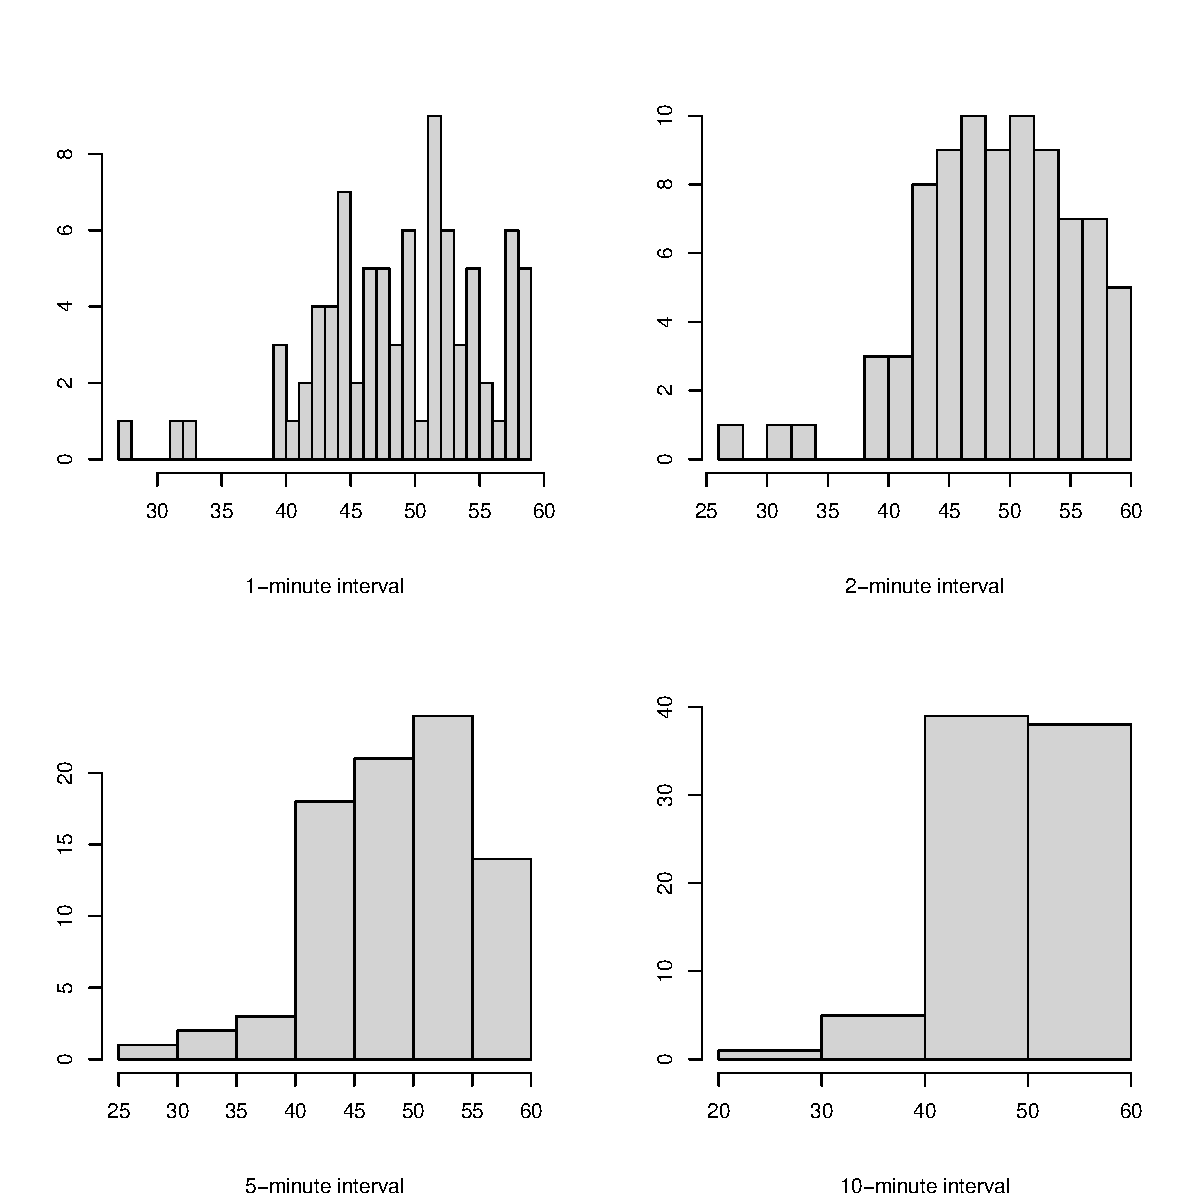
\includegraphics[width=0.8\linewidth]{image/Chap5_continuous_rv.pdf}
    \caption{学生到达教室的直方图}
    \label{fig:chap05_continuous_rv}
\end{figure}
\end{instance}

我们发现,时间是连续的,且$X$的取值可以充满$(0,60)$这个区间。于是,$X$就是一个连续型随机变量。当我们不断细化间隔的划分,在同一时刻到达教室的学生不会超过1人。于是,利用概率分布列$P(X=x)$来刻画$X$是不恰当的。所以,我们需要提出一个新的概念——概率密度函数。


\section{概率密度函数}
概率密度函数$p(x)$的值虽不是概率,但乘微分元$\text{d} x$就可以得小区间$(x,x+\text{d}x)$上概率的近似值,即
$$
p(x)\text{d}x = P(x<X<x+\text{d}x).
$$
在$(a,b)$上很多相邻的微分元的累积就得到$p(x)$在$(a,b)$上的积分,这个积分值就是$X$在$(a,b)$上取值的概率,即
$$
\int_{a}^b p(x)\text{d}x = P(a<X<b).
$$
特别,在$(-\infty,x]$上$p(x)$的积分就是分布函数$F(x)$,即
$$
\int_{-\infty}^x p(t)\text{d} t = P(X\leq x)=F(x).
$$
这一关系式是连续随机变量$X$的概率密度函数$p(x)$最本质的属性。

\begin{definition}{概率密度函数}\label{def:pdf}
    设随机变量$X$的分布函数为$F(x)$,如果存在实数轴上的一个非负可积函数$p(x)$,使得对任意实数$x$有
$$F(x) = \int_{-\infty}^{x} p(t) d t,$$
那么称$p(x)$为$X$的概率密度函数(probability density function, p.d.f.)。称随机变量$X$为连续型随机变量,其分布函数$F(x)$是连续分布函数。
\end{definition}
\begin{property}
连续型随机变量$X$的概率密度函数$p(x)$,其具有
\begin{enumerate}
    \item 非负性\quad $p(x) \geqslant 0$;
    \item 正则性 \quad  $\int_{-\infty}^{\infty} p(x) d x$。
\end{enumerate}
\end{property}
\begin{remark}
上述两条也是判别某个函数是否为密度函数的充要条件。
\end{remark}
\begin{example}
向区间$(0,a)$上任意投点,用$X$表示其坐标。设这个点落在$(0,a)$中任一小区间的概率与这个小区间的长度成正比,而与小区间位置无关。求$X$的分布函数和密度函数。
\end{example}
\begin{solution}
记$X$的分布函数为$F(x)$,则
\begin{itemize}
\item 当$x<0$时,因为$\{X \leq x\}$是不可能事件,所以$F(x)=P( X \leq x)=0$;
\item 当$x \geq a$时,因为$\{X \leq x\}$是必然事件,所以$F(x)=P( X \leq x)=1$;
\item 当$0 \geq x <a $ 时, $F(x) =P(X \leq x)=P(0 \leq X \leq x) = k x$,其中$k$为比例系数。因为$F(a)=ka$,所以$k = \frac{1}{a}$。于是,分布函数为$$F(x)=\left\{\begin{aligned}
    0, &\quad  x<0 \\
\frac{x}{a}, & \quad 0 \leq x<a \\
1, &\quad  x \geq a.
\end{aligned}\right.
$$
\end{itemize}
令$X$的密度函数$p(x)$,
\begin{itemize}
    \item 当$x<0$或$x>a$时,$p(x)=F'(x)=0$;
    \item 当$x>a$时,$p(x)=F'(x)=0$,
    \item 当$0< x< a$,$$
    p(x) = F'(x) =  \frac{1}{a}.
    $$
\end{itemize}
而在$X=0$和$x=a$处,$p(x)$可取任意值,一般就近取值为宜,这不会影响概率的计算。于是,$X$的概率密度是
$$
p(x)= \left\{\begin{aligned}
\frac{1}{a}, &\quad  0<x<a \\
0, & \quad \text { 其他 }
\end{aligned}\right.
$$
\end{solution}
\begin{remark}
    这个分布就是区间$(0,a)$上的均匀分布,记$U(0, a)$。
\end{remark}

\begin{example}
验证$$f(x)=\left\{\begin{aligned}
\frac{1}{2 \sqrt{x}}, &\quad  0<x<1 \\
0, & \quad \text { 其他 }
\end{aligned}\right.$$
是否为一个随机变量$X$的概率密度函数?\\
\end{example}
\begin{solution}
    【思路】验证$f(x)$是否满足非负性和正则性。具体证明过程由同学们课后证明。
    \vspace{3cm}
\end{solution}
\begin{remark}
    比较密度函数与分布列的异同:
    \begin{enumerate}
 \item 已知概率分布列或概率密度函数,可以求出概率分布函数或概率值;
 \item 离散随机变量的分布函数$F(x)$总是右连续的阶梯函数;而连续随机变量的分布函数$F(x)$一定是整个数轴上的连续函数,
 其增量为
$$F(x+\Delta x)-F(x)=\int_{x}^{x+\Delta x} p(t) d t \rightarrow 0(\Delta x \rightarrow 0).$$
 \item  离散型随机变量$X$在其可能取值的点$x_1,x_2,...,x_n,...,$上的概率不为$0$,而连续随机变量$X$在($-\infty,+\infty$)上任一点$a$的概率恒为$0$, 即 $P(x=a)=\int_{a}^{a} p(x) d x=0 $。这可以作为以下观点的一个例子:不可能事件的概率为$0$,但概率为$0$的事件不一定是不可能事件。类似地,必然事件的概率为$1$,但概率为1的事件不一定是必然事件。
 \item 连续型随机变量$P(a \leq X \leq b)=P(a<X \leq b)=P(a \leq X<b)=P(a<X<b)$,但离散型随机变量并不满足这个性质,要“点点计较”。
\item 由于在若干点上改变概率密度函数$p(x)$的值并不影响其积分值,从而不影响分布函数$F(x)$的值。这意味着一个连续分布的密度函数不唯一。
\end{enumerate}
\end{remark}
\section{常见的连续随机变量}
\subsection{均匀分布}
\begin{definition}\label{def:uniform_dist}
设定义在区间$(a,b)$的一个随机变量$X$,其中$a<b$为两个未知参数。$X$的概率密度函数为
$$
p(x) = \frac{1}{b-a}, a< x<b.
$$
称$X$的分布为均匀分布。记$X\sim U(a,b)$。
\end{definition}

\subsection{正态分布}
\begin{definition}\label{def:normal_dist}
设定义在区间$(-\infty,\infty)$的一个随机变量$X$。$X$的概率密度函数为
$$
p(x) =\frac{1}{\sqrt{2\pi \sigma^2}}\exp\left\{-\frac{1}{2\sigma^2} (x-\mu)^2\right\}, x \in R.
$$
称$X$的分布为正态分布。记$X\sim N(\mu,\sigma^2)$,其中参数$\mu \in R, \sigma^2 >0$。
\end{definition}
\begin{remark}
    \begin{enumerate}
        \item 正态分布是最早由法国数学家棣莫弗(Abraham de Moivre)在近似二项分布时得到的,后由德国数学家高斯(Carolus Fridericus Gauss)在测量误差时导出。因高斯的工作对后世的贡献巨大,所以,正态分布又称{\bf 高斯分布}。
        \item 概率密度函数$p(x)$是一条钟型曲线,特点为:中间高,两边低,左右对称。
        \item 正态分布的两个参数$\mu$和$\sigma^2$是决定密度函数位置和形状,称$\mu$为位置参数,$\sigma^2$是尺度参数。
    \end{enumerate}
\end{remark}
这里很自然我们构建一个正态分布类,即
$$
\mathcal{P} = \{N(\mu,\sigma^2):\mu \in R, \sigma^2 >0\}.
$$
其中有个极为特殊的正态分布——标准正态分布,即$\mu = 0,\sigma^2 = 1$。这里我们具体讲解一下这个特殊的正态分布。

\begin{remark}
    \begin{enumerate}
        \item 标准正态分布的密度函数为
        $$
        \phi(z) = \frac{1}{\sqrt{2\pi}} \exp\left\{-\frac{1}{2}z^2\right\};
        $$
        \item 标准正态分布的分布函数为
        $$
        \Phi(z) = \int_{-\infty}^z \phi(x)\text{d} x;
        $$
        \item 标准正态分布的概率计算常用公式:
        \begin{enumerate}
       \item $\Phi (-z)=P(Z\le -z)=P(Z\ge z)=1-\Phi(z)$
       \item $P(Z>z)=1-\Phi(z)$
       \item $P(a<Z<b)=\Phi(b)-\Phi(a)$
       \item $P(\left | Z \right | <c)=2\Phi(c)-1, (c\ge 0)$\\
    \end{enumerate}
    \end{enumerate}
\end{remark}
    \begin{theorem}\label{property:standard_normal}
  若随机变量$X\sim N(\mu,\sigma^{2})$,则$Z=\frac{x-\mu }{\sigma } \sim N(0,1)$.
  \end{theorem}
   \begin{proof}
   记$X$和$Z$的分布函数分别为$F_{X}(x)$和$F_{Z}(z)$,密度函数分别为$p_{X}(x)$和$p_{Z}(z)$.\\
   则由分布函数的定义可知
   \begin{equation}
   \begin{aligned}
   F_{Z}(z)
   &=P(Z\le z)\\
   &=P(\frac{X-\mu }{\sigma } \le z)\\
   &=P(X\le \mu +\sigma \mu )\\
   &=F_{X} (\mu +\sigma \mu )\\
   \end{aligned}
   \end{equation}
   由于正态分布函数是严格单调递增且处处可导。因此
   \begin{equation}
   \begin{aligned}
   p_{Z}(z)
   &=\frac{\mathrm{d}}{\mathrm{d} z} F_{Z}(z)\\
   &=\frac{\mathrm{d}}{\mathrm{d} z} F_{X}(\mu +\sigma z)\\
   &= p_{X}(\mu +\sigma z)\cdot \sigma \\
   &=\frac{1}{\sqrt{2\pi \sigma ^{2}} } e^{-\frac{1}{2\sigma ^{2}}(\mu +\sigma z -\mu )^{2} }\cdot \sigma \\
   &=\frac{1}{\sqrt{2\pi } } e^{-\frac{z^{2}}{2} }\\
  \end{aligned}
  \end{equation}
  由此可得$$U=\frac{x-\mu }{\sigma } \sim N(0,1)$$
  \end{proof}
  \begin{remark}
  $3\sigma$原则:
      \begin{enumerate}
          \item   $P(\mu -\sigma <X<\mu +\sigma )=2\Phi(1)-1\approx 0.6826$;
          \item 
  $P(\mu -2\sigma <X<\mu +2\sigma )=2\Phi(2)-1\approx 0.9545$;
  \item 
  $P(\mu -3\sigma <X<\mu +3\sigma )=2\Phi(3)-1\approx 0.9973$。
      \end{enumerate}
  \end{remark}  
 
\subsection{指数分布}
\begin{definition}\label{expential_dist}
    设一随机变量$X$,其密度函数为
    $$p(x)=\left\{\begin{matrix}
    \lambda e^{-\lambda x} ,&x\ge 0 \\
    0,&x<0
    \end{matrix}\right.$$
    则称$X$的分布为指数分布,记$X\sim Exp(\lambda)$,其中参数$\lambda>0$。
\end{definition}
根据随机变量的密度函数,可以计算其分布函数为
\begin{eqnarray*}
F_{X} (x) =  \left\{\begin{matrix}
    \int_{0}^{x}p(t)dt=\int_{0}^{x}\lambda e^{-\lambda t} dt= e^{-\lambda t}|_{0}^{x} =1-e^{-\lambda x}  ,&x\ge 0 \\
    0,&x<0
    \end{matrix}\right.
\end{eqnarray*}
类似于几何分布,指数分布也具有无记忆性。
\begin{theorem}[(指数分布的无记忆性)]\label{property:no_memory_expential}
    如果随机变量$X\sim Exp(\lambda)$,则对任意$s>0,t>0$有$$P(X>t+s|X>s)=P(X>t).$$
\end{theorem}
\begin{proof}
因为$X\sim Exp(\lambda)$,所以$P(X>s)=e^{-\lambda s},s>0$。又因为$\left \{ X>s+t \right \} \subset \left \{ X>s \right \} $,于是,条件概率$$P(X>s+t|X>s)=\frac{P(X>s+t)}{P(X>s)}=\frac{e^{-\lambda (s+t)} }{e^{-\lambda s} }=e^{-\lambda t}.$$
    \end{proof}
泊松分布与指数分布有非常紧密的关系,我们利用以下一个例子来说明。
\begin{example}
    如果某设备在长为$t$的时间$(0,t) $内发生故障的次数$N(t)$(与时间长度$t$有关)服从参数为$\lambda t$的泊松分布,且$N(0)=0$,则从$0$时开始首次发生故障的时间$T$服从参数为$\lambda$的指数分布。
\end{example}
\begin{solution}
    设$N(t)\sim P(\lambda t)$,即$$P(N(t)=k)=\frac{(\lambda t)^{k} }{k!} e^{-\lambda t} ,k=0,1,\cdots $$
    注意到从$0$时开始首次发生故障的时间$T$是非负随机变量且事件$\left \{ T\geq t \right \} $说明此设备在$\left [ 0,t \right ]$内没有发生故障。即$\left \{ T\geq t \right \} =\left \{ N(t)=0 \right \} .$由此可得,
    \begin{itemize}
    \item 当$t<0$时,有$$F_{T} (t)=P(T\le t)=0;$$
    \item  当$t\geq 0$时,有$$F_{T} (t)=P(T\le t)=1-P(T> t) = 1-P(T\geq t)=1-P(N(t)=0)=1-e^{-\lambda t} .$$
    \end{itemize}
    因此,$T\sim {Exp}(\lambda)$,即从$0$时开始首次发生故障的时间$T$服从参数为$\lambda$的指数分布。
\end{solution}
\subsection{伽马分布}
\begin{definition}
    称
    $$\Gamma (\alpha )=\int_{0}^{+\infty } x^{\alpha -1} e^{-x} dx,\alpha >0$$
    为伽马函数。
\end{definition}
根据伽马函数的定义,可以证明伽马函数的一些常用性质。
\begin{property}
    \begin{enumerate}
        \item $\Gamma (1 )=1, \quad \Gamma (\frac{1}{2}  )=\sqrt{\pi } $;
        \item $\Gamma (\alpha +1 )=\alpha \Gamma(\alpha ), \quad \text{特别地,}\Gamma (n+1 )=n\Gamma(n)=n!$。
    \end{enumerate}
    \end{property}
    \begin{proof}
    \begin{enumerate}
        \item 令$x=u^{2}$,于是,
        \begin{eqnarray*}
            \Gamma \left(\frac{1}{2} \right)&=&\int_{0}^{+\infty } x^{-\frac{1}{2} } e^{-x} dx\\
            &=&\int_{0}^{+\infty } u^{-1} e^{-u^{2}}d(u^{2} ) \\
            &=& 2\int_{0}^{+\infty }e^{-u^{2}}du\\
            &=& \int_{-\infty }^{+\infty} e^{-u^{2}}du\\
            &=& \int_{-\infty }^{+\infty}\frac{1}{\sqrt{2\pi \cdot \frac{1}{2} } } e^{-\frac{u^{2} }{2(\frac{1}{2} )} }du\cdot \sqrt{\pi }\\
            &=& \sqrt{\pi }.
       \end{eqnarray*}
        \item 这里只需要证明$\Gamma (\alpha +1 )=\alpha \Gamma(\alpha )$,即
        \begin{eqnarray*}
            \Gamma (\alpha +1)
           &=&\int_{0}^{+\infty} x^{\alpha } e^{-x} dx\\
           &=&\int_{0}^{+\infty} \left ( -x^{\alpha }  \right ) d\left ( e^{-x}  \right ) \\
           &=&-x^{\alpha }e^{-x}|_{0}^{+\infty } +\int_{0}^{+\infty} e^{-x} d\left ( x^{\alpha } \right ) \\
           &=&\int_{0}^{+\infty} \alpha x^{\alpha-1 }e^{-x} dx\\
           &=&\alpha \Gamma(\alpha ).
        \end{eqnarray*}
    \end{enumerate}   
    \end{proof}
    
    基于伽马函数,我们来定义伽马分布。
    \begin{definition}\label{def:gamma_distribution}
        假设$X$为一随机变量,其密度函数为
        $$
        p(x)=\left\{\begin{matrix}
    \frac{\lambda ^{\alpha } }{\Gamma (\alpha )}x^{\alpha -1}e^{-\lambda x}  & ,x\ge 0\\
    0&,x<0
    \end{matrix}\right.
        $$
        则称其分布为伽马分布,记作$X\sim Ga(\alpha,\lambda)$,其中$\alpha>0$为形状参数,$\lambda>0$为尺度参数。
    \end{definition}
    \begin{remark}
        当$\alpha = 1$时,$Ga(1,\lambda)=e^{\lambda}$。
    \end{remark}
    以下例子讲解了泊松分布与伽马分布之间的关系,和之前讲解过的关于泊松分布与指数分布之间的关系的证明过程类似,供学生课后自学。
    \begin{example}
        若在$(0,t)$内发生冲击的次数$N(t)$服从参数为$\lambda t$的泊松分布,试证明第$n$次冲击来到的时间$S_{n}$服从伽马分布$Ga(n,\lambda)$。
    \end{example}
     \begin{proof}
    因为事件“第$n$次冲击来到的时间$S_{n}$小于等于$t$”等价于事件“$(0,t)$内发生冲击的次数$N(t)$大于等于$n$”,即$$\left \{ S_{n} \le t \right \} =\left \{ N(t)\ge n \right \}. $$
    于是,$S_{n}$的分布函数为$$F(t)=P(S_{n}\le t )=P(N(t)\ge n)=\sum_{k=n}^{+\infty } \frac{(\lambda t)^{k} }{k!} e^{-\lambda t}.$$
    令$a_{k} = \frac{(\lambda t)^{k} }{k!} e^{-\lambda t}$, $ b_{k} = \frac{\lambda ^{k} }{\Gamma (k)}\int_{t}^{+\infty }x^{k-1}e^{-\lambda x}dx $。
    由于
    \begin{eqnarray*}
         b_{k}
       &=&\frac{\lambda ^{k} }{\Gamma (k)}\int_{t}^{+\infty }x^{k-1}e^{-\lambda x}dx \\
       &=&\frac{\lambda ^{k} }{(k-1)!}\int_{t}^{+\infty }-\frac{1}{\lambda } x^{k-1}d e^{-\lambda x}  \\
       &=&\frac{\lambda ^{k} }{(k-1)!}(-\frac{1}{\lambda } x^{k-1}e^{-\lambda x} |_{t}^{+\infty } +\frac{k-1}{\lambda }\int_{t}^{+\infty }x^{k-2} e^{-\lambda x}dx   )\\
       &=&\frac{\lambda ^{k} }{(k-1)!}(\frac{1}{\lambda } t^{k-1}e^{-\lambda t}  +\frac{k-1}{\lambda }\int_{t}^{+\infty }x^{k-2} e^{-\lambda x}dx   )\\
       &=&\frac{\lambda ^{k-1} }{(k-1)!} t^{k-1}e^{-\lambda t}  +\frac{\lambda ^{k-1} }{(k-2)!}\int_{t}^{+\infty }x^{k-2} e^{-\lambda x}dx  \\
       &=&a_{k-1} +b_{k-1}
    \end{eqnarray*}
    可得$a_{k-1} =b_{k}-b_{k-1}$,则
    \begin{eqnarray*}
        \sum_{k=1}^{n-1} a_{k} &=&\sum_{k=1}^{n-1}(b_{k+1}-b_{k})\\
        &=&(b_{2}-b_{1})+\cdots +(b_{n}-b_{n-1})=b_{n}-b_{1}\\
        &=&\frac{\lambda ^{n} }{\Gamma (n)}\int_{t}^{+\infty } x^{n-1}e^{-\lambda x} dx-a_{0} .
    \end{eqnarray*}  且
    \begin{eqnarray*}
        b_{1} &=&\frac{\lambda  }{\Gamma (1)}\int_{t}^{+\infty } e^{-\lambda x} dx\\
        &=&\lambda \int_{t}^{+\infty } e^{-\lambda x} dx\\
        &=&-e^{-\lambda x}|_{t}^{+\infty }=e^{-\lambda t}=a_{0} \\
         \end{eqnarray*}
    由此,我们有
    $$\sum_{k=0}^{n-1 } \frac{(\lambda t)^{k} }{k!} e^{-\lambda t}= \frac{\lambda ^{n} }{\Gamma (n)}\int_{t}^{+\infty } x^{n-1}e^{-\lambda x} dx
   $$
    因此,
    \begin{eqnarray*}
       F(t)
       &=&\sum_{k=n}^{+\infty } \frac{(\lambda t)^{k} }{k!} e^{-\lambda t}\\
       &=&1-\frac{\lambda ^{n} }{\Gamma (n)}\int_{t}^{+\infty }  x^{n-1} e^{-\lambda x} dx\\
       &=&1-\int_{t}^{+\infty }  \frac{\lambda ^{n} }{\Gamma (n)}x^{n-1} e^{-\lambda x} dx\\
       &=&\int_{0}^{t}  \frac{\lambda ^{n} }{\Gamma (n)}x^{n-1} e^{-\lambda x} dx
    \end{eqnarray*}
    所以,$S_{n}\sim Ga(n,\lambda)$.
    \end{proof}
\subsection{贝塔分布}
\begin{definition}
    称
    $$B(a,b)=\int_{0}^{1} x^{a-1} (1-x)^{b-1} dx,a>0,b>0$$
    为贝塔函数。
\end{definition}
根据贝塔函数的定义,可以证明贝塔函数的一些常用性质。
 \begin{property}
    \begin{enumerate}
        \item  \item $B(a,b)=B(b,a)$;
        \item $B(a,b)=\frac{\Gamma (a)\Gamma (b)}{\Gamma (a+b)} $。
    \end{enumerate}
    \end{property}
    \begin{proof}
    由伽马函数的定义可知$$\Gamma (a)\Gamma (b)=\int_{0}^{+\infty } \int_{0}^{+\infty } x^{a-1} y^{b-1} e^{-(x+y)} dxdy.$$
    作变量变换$$\left\{\begin{matrix}
    x=uv\\
    y=u(1-v)
    \end{matrix}\right.\Longrightarrow 
    \left\{\begin{matrix}
    u=x+y\\
    v=\frac{u}{x} 
    \end{matrix}\right.\Longrightarrow
    J=\begin{vmatrix}
    v&u \\
    (1-v)&-u
    \end{vmatrix}=-u$$故
    \begin{eqnarray*}
         \Gamma (a)\Gamma (b)
       &=&\int_{0}^{1 } \int_{0}^{+\infty } (uv)^{a-1} (u(1-v))^{b-1} e^{-u} ududv\\
       &=& \int_{0}^{+\infty } u^{a+b-1}e^{-u}du  \cdot \int_{0}^{1 }v^{a-1}(1-v)^{b-1}dv\\
       &=&\Gamma (a+b)B(a,b).
    \end{eqnarray*}
    \end{proof} 
    基于贝塔函数,我们来定义贝塔分布。
   \begin{definition}
       假设一随机变量$X$,其密度函数为$$p(x)=\left\{\begin{matrix}
    \frac{\Gamma (a+b)}{\Gamma (a)\Gamma (b)}x^{a-1} (1-x)^{b-1},  &0<x<1, \\
    0,& \text{其他}.
    \end{matrix}\right.$$
    则称$X$的分布为贝塔分布,记$X\sim Be(a,b)$,其中$a>0,b>0$均为形状参数。
   \end{definition}
   \begin{remark}
       特别地,当$a=1,b=1$时,$Be(1,1) = U(0,1)$。
   \end{remark}
   \section{习题}

        \begin{enumerate}
            \item Alvin向半径为r的圆形目标投掷飞镖,有可能落到目标中的任何一点。设X为Alvin的飞镖的落点与目标中心的距离。
            \begin{enumerate}
                \item 计算$X$的概率密度函数;
\item 目标具有半径为$t$的内圆。如果 $X\leq t$,Alvin 得到 $S = 1/X$ 的分数。 否则他的分数为$S = 0$。 求 S 的 分布函数。同时,S 是连续随机变量吗?
            \end{enumerate}
\item 设连续随机变量$X$的分布函数为
$$
F(x) = \left\{\begin{matrix}0, & x<0,\\
    	Ax^2, & 0\leq x < 1,\\
    	1, & x \geq 1.
    	\end{matrix}
    	 \right.
$$
试求:
\begin{enumerate}
    \item 系数$A$;
    \item $X$落在区间$(0.3,0.7)$内的概率;
\item $X$的密度函数;
\end{enumerate}

\item 设连续随机变量$X$的密度函数$p(x)$是一个偶函数,$F(x)$为$X$的分布函数,求证对任意实数$a > 0$,有
\begin{enumerate}
    \item $F(-a) = 1- F(a) = 0.5-\int_0^a p(x)dx$;
\item  $P(|X| < a) = 2F(a)-1$;
\item  $P(|x| > a) = 2(1-F(a))$。
\end{enumerate}

\item  设$K$服从$(1,6)$上的均匀分布,求方程$x^2 + Kx +1 = 0$有实根的概率。

\item 设随机变量$X$服从伽马分布$Ga(2,0.5)$,试求$P(X < 4)$。

\item  某地区漏缴税款的比例$X$服从参数$a=2,b=9$的贝塔分布,试求此比例小于$10\%$的概率及平均漏缴税款的比例。

\item  假设一个随机变量$X$,其概率质量函数或概率密度函数(统称为概率函数)为$p(x)$。设$g(x)$为一个非常值函数。如果存在一个非零常数$c$,使得
$$
p(x) = c \cdot g(x)
$$
那么称$g(x)$为概率函数的“核”。
例如:$X\sim N(0,1)$,其概率函数的“核”为$\exp\{-x^2/2\},x \in R$;$X\sim b(1,p)$,其概率函数的“核”为$p^{x}(1-p)^{1-x},x = 0,1$;

请指出以下函数是哪个随机变量的概率函数的核。
\begin{enumerate}
    \item $p^{x}(1-p)^{m-x}, x=0,1,2,\cdots,m$,其中$p,m$是参数。
    \item $p^{m}(1-p)^{x-m}, x=m,m+1,\cdots$,其中$p,m$是参数。
    \item $x^{p}(1-x)^{m-p},x\in (0,1)$;这里$p,m$是参数。
\item $e^{-2\gamma x^2},x\in R$,这里$\gamma$是参数。
\item $e^{-2\gamma x},x\in R$,这里$\gamma$是参数。
\item $x^{2}e^{-2\gamma x},x\in R$,这里$\gamma$是参数。
\end{enumerate}
        \end{enumerate}
% \begin{exercise}
% \end{exercise}